\documentclass[10pt]{article}
\usepackage{icmlko}

\icmlmeta{IP 파운데이션 월드모델}{110}{빼면 더 잃는다}{팝업이 안 따라오는 이유를 ``사람이 매긴 축''에서 찾았는데 빼 보니 $-$0.0727이었다 --- 가설은 죽었고, 노트 109의 되돌림은 악화 4/4로 옳았다}

\begin{document}

\twocolumn[
\icmlheader

\begin{abstract}
두 가지를 했다. \textbf{① 되돌림 검정.} 노트 109는 점추정만 보고 세 도메인
채우기를 되돌렸다. 짝지은 붓스트랩으로 검정하니 다섯 채우기가 두 채우기보다
$\Delta-$0.0074이고 \textbf{씨앗 넷 전부 구간이 0 아래}
($-$0.0122$\sim-$0.0008)다 --- \textbf{악화 4/4. 되돌린 것이 옳았다.}
팝업은 $+$0.0040 보류라 되돌림이 제품을 해치지도 않는다. \textbf{② 팝업 가설.}
노트 106--109에서 네 번 팝업이 안 따라왔고, 팝업만 열 축이 전부 \emph{사람이
기획서를 읽고 매긴 것}이라는 점을 의심했다 --- 노트 108이 정렬에 넣은 두 축이
팝업에서는 사람 판단이고 남에서는 가격표와 링크 개수다. \textbf{팝업의 그 두
축을 정렬에서 빼 봤다. 팝업이 더 떨어진다} --- 둘 다 빼면 $-$0.0293,
\textbf{입장료만 빼도 $-$0.0727}이다. \textbf{가설이 죽었다.} 대조도 방향이
같다 --- 아이돌의 둘을 빼면 팝업 $-$0.0148, 애니의 둘을 빼면 $+$0.0059로
작다. 대신 왜 팝업이 다른지는 보인다. 팝업에서 새 두 축은 옛 셋과 \textbf{크게
얽혀 있다} --- 미디어 홍보 $\leftrightarrow$ 굿즈 규모 $+$0.488, 입장료
$\leftrightarrow$ 타깃 폭 $+$0.388. 만화 · 세계애니에서는 최대가 $+$0.35다.
\textbf{팝업에서는 다섯 축이 세 축의 확장이 아니라 세 축을 보강하는 구조}이고,
그래서 빼면 크게 잃는다. 끝으로 \textbf{서술을 고친다} --- ``팝업이 네 노트째
안 따라온다''는 과했다. 전체 자료에서 팝업은 $+$0.4501에서 $+$0.4601로
\textbf{올랐다}(보류지만 양수). 음수인 것은 시간 분할뿐이고, 그 이유는 노트
106이 이미 밝혔다 --- \textbf{팝업엔 과거가 없다.}
\end{abstract}
]

\begin{figure*}[t]
\centering
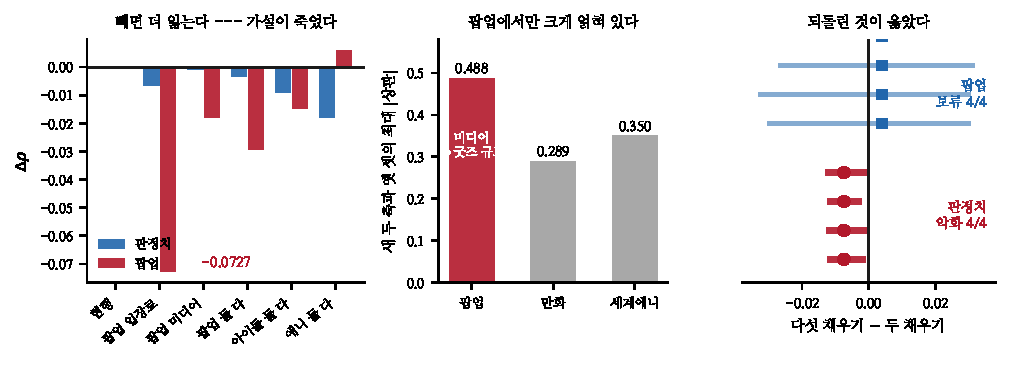
\includegraphics[width=\textwidth]{figs/pk.pdf}
\caption{왼쪽 --- 빼면 더 잃는다. 가운데 --- 팝업에서만 크게 얽혀 있다.
오른쪽 --- 되돌린 것이 옳았다.}
\end{figure*}

\section{되돌림이 옳았다}

\begin{table}[t]
\centering\tsize
\caption{다섯 채우기 $-$ 두 채우기. 씨앗 넷 · 짝지은 붓스트랩 100회.}
\begin{tabular}{lrll}
\toprule
& $\Delta$ & 95\% 구간 & \\
\midrule
\multicolumn{4}{l}{\emph{판정치}} \\
20260729 & $-$0.0074 & $-$0.0117 $\sim$ $-$0.0018 & \textbf{악화} \\
19770101 & $-$0.0074 & $-$0.0117 $\sim$ $-$0.0008 & \textbf{악화} \\
20250315 & $-$0.0074 & $-$0.0115 $\sim$ $-$0.0031 & \textbf{악화} \\
20260101 & $-$0.0074 & $-$0.0122 $\sim$ $-$0.0013 & \textbf{악화} \\
\midrule
\multicolumn{2}{l}{\emph{팝업}} & $+$0.0040 & 보류 4/4 \\
\bottomrule
\end{tabular}
\end{table}

\claimx{노트 109의 되돌림이 옳았다 --- 게임 · 웹툰 · 도서까지 채우면
\textbf{악화 4/4}다. 그리고 되돌림이 제품을 해치지도 않는다(팝업 $+$0.0040
보류).}{되돌린 자료는 버리지 않고 \texttt{media\_push\_fill\_all.json} 에
뒀다. 같은 개념으로 다시 채울 길이 생기면 쓸 수 있다.}

\section{팝업 가설을 세우고 죽였다}

팝업에는 아홉 도메인에 없는 성질이 있다.

\begin{quote}\fontsize{9.5}{11.5}\selectfont
\textbf{팝업} --- 열 축 전부 사람이 기획서를 읽고 매긴 것\\
\textbf{나머지 아홉} --- 전부 플랫폼 메타에서 규칙으로 유도한 것
\end{quote}

노트 108이 정렬에 넣은 두 축이 팝업에서는 사람 판단이고 남에서는 가격표 ·
링크 개수다. \textbf{같은 슬롯에 다른 종류의 측정이 들어 있으면} 프로크루스테스가
헛돈다는 것이 가설이었다.

\begin{table}[t]
\centering\tsize
\caption{정렬에서 빼 본다.}
\begin{tabular}{lrr}
\toprule
& $\Delta$판정치 & $\Delta$팝업 \\
\midrule
현행(공통 다섯) & --- & --- \\
\textbf{팝업의 입장료만 끄기} & $-$0.0067 & \textbf{$-$0.0727} \\
팝업의 미디어만 끄기 & $-$0.0007 & $-$0.0178 \\
팝업의 둘 다 끄기 & $-$0.0032 & $-$0.0293 \\
\midrule
아이돌의 둘 다 끄기(대조) & $-$0.0089 & $-$0.0148 \\
애니의 둘 다 끄기(대조) & $-$0.0178 & $+$0.0059 \\
\bottomrule
\end{tabular}
\end{table}

\claimx{\textbf{가설이 죽었다.} 팝업의 사람이 매긴 두 축을 정렬에서 빼면 팝업이
$-$0.0293 떨어지고, 입장료만 빼도 \textbf{$-$0.0727}이다. 팝업은 그 축들이
\emph{있어야} 한다 --- 사람이 매긴 것이 정렬을 방해하고 있지 않다.}
{끄면 팝업의 인자 공간도 얇아진다(노트 98의 가짜약 문제). 다만 아이돌 ·
애니를 끌 때는 팝업이 $-$0.0148 · $+$0.0059로 작으므로, 팝업 자신을 끄는
$-$0.0727은 그 효과로 다 설명되지 않는다.}

\section{대신 얽힘이 보인다}

\begin{table}[t]
\centering\tsize
\caption{새 두 축과 옛 공통 셋의 순위 상관.}
\begin{tabular}{llrrr}
\toprule
& & 타깃 폭 & 굿즈 규모 & 매장 노출 \\
\midrule
\textbf{팝업} & 입장료 & \textbf{$+$0.388} & $-$0.153 & $+$0.205 \\
& 미디어 & $+$0.117 & \textbf{$+$0.488} & $+$0.109 \\
\midrule
만화 & 입장료 & $+$0.279 & $+$0.044 & $+$0.289 \\
& 미디어 & $+$0.277 & $+$0.262 & $+$0.171 \\
세계애니 & 입장료 & $+$0.264 & $+$0.152 & $+$0.037 \\
& 미디어 & $+$0.350 & $+$0.234 & $+$0.155 \\
\bottomrule
\end{tabular}
\end{table}

\claimx{팝업에서만 새 축이 옛 축과 크게 얽혀 있다($+$0.488 · $+$0.388).
만화 · 세계애니는 최대가 $+$0.35다. \textbf{팝업에서는 다섯 축이 세 축의
\emph{확장}이 아니라 \emph{보강}}이고, 그래서 빼면 크게 잃는다.}{얽힘이
크면 중복이라 빼도 될 것 같은데 반대다. 얽힘이 정렬을 \emph{안정시키는}
경로가 있을 수 있는데 확인 안 했다.}

\section{서술을 고친다}

노트 109까지 ``팝업이 네 노트째 안 따라온다''고 적었다. \textbf{과했다.}

\begin{table}[t]
\centering\tsize
\caption{팝업의 실제 궤적.}
\begin{tabular}{lrr}
\toprule
& 전체 자료 & 시간 분할 \\
\midrule
노트 105(입장료) & $+$0.0070 & 음수 3/3 \\
노트 108(채택) & \textbf{$+$0.0100} & $-$0.0350 \\
노트 109(되돌림 뒤) & \textbf{$+$0.4601} & --- \\
\bottomrule
\end{tabular}
\end{table}

\claimx{전체 자료에서 팝업은 $+$0.4501에서 $+$0.4601로 \textbf{올랐다} ---
보류이지만 양수다. 음수인 것은 \emph{시간 분할}뿐이고 그 이유는 노트 106이
이미 밝혔다: \textbf{팝업엔 과거가 없다}($T{=}2023$ 에 0건, 2024 에 1건).}
{그래도 시간 분할이 더 정직한 규약이다. ``전체 자료에서 올랐다''로 안심하면
안 된다 --- 제품은 미래를 맞히는 것이다.}

\begin{quote}\fontsize{9.5}{11.5}\selectfont
자기 정정이 이 프로젝트의 습관이 됐다 --- 노트 83(라벨 신뢰도) · 87(무라벨
전제) · 102(자기 지침) · 109(자기 공)에 이어 다섯 번째다. \textbf{이번 것은
서술의 과장이지 계산의 오류가 아니다.} 그래도 적어 둔다. 네 노트에 걸쳐
``안 따라온다''를 반복하면 그것이 사실이 된다.
\end{quote}

\section{한계}

\begin{itemize}[leftmargin=1.1em,itemsep=0.15em]
\item \textbf{팝업이 시간 분할에서 왜 내리는지는 여전히 모른다.} 가설 하나를
      죽였을 뿐이다.
\item 축을 끄면 인자 공간도 얇아진다 --- 노트 98이 지적한 가짜약 문제가
      여기서도 완전히 해소되지 않는다.
\item 얽힘($+$0.488)이 왜 도움이 되는지 설명 못 한다.
\item 되돌림 검정에서 두 설정의 복원추출 색인을 공유했다. 도메인 크기가 같아
      대응이 맞지만 코드로만 확인했다.
\item 텀블벅 · 펀딩은 여전히 0\%다.
\end{itemize}

\section{다음}

\begin{enumerate}[leftmargin=1.3em,itemsep=0.15em]
\item \textbf{시간 분할의 팝업을 직접 판다} --- 어느 \emph{출처}에서 오는
      전이가 나빠지는지 쌍별로 본다. 노트 97의 기제 표와 같은 형식으로.
\item \textbf{팝업 레코드} --- 노트 92 · 106 · 107 · 110이 전부 같은 곳을
      가리킨다. 510건이면 설계 판정이 되고, 그때 시간 분할도 안정된다.
      \textbf{모을 방법을 설계한다.}
\item 얽힘이 정렬을 안정시키는가 --- 다른 도메인에 인위로 얽힘을 만들어 본다.
\item 텀블벅 API. 펀딩만 남았다.
\end{enumerate}

\vspace{0.6em}
\hrule height 0.3pt
\vspace{0.5em}
{\footnotesize
\textbf{참고문헌}\\[0.3em]
Meredith, W. (1993). Measurement invariance, factor analysis and factorial
invariance. \emph{Psychometrika}, 58(4), 525--543.\\[0.15em]
Schoenemann, P. H. (1966). A generalized solution of the orthogonal Procrustes
problem. \emph{Psychometrika}, 31(1), 1--10.\\[0.15em]
Efron, B., Tibshirani, R. J. (1993). \emph{An Introduction to the Bootstrap}.
Chapman \& Hall.\\[0.15em]
Bergmeir, C., Benitez, J. M. (2012). On the use of cross-validation for time
series predictor evaluation. \emph{Information Sciences}, 191, 192--213.\\[0.15em]
Ben-David, S. et al. (2010). A theory of learning from different domains.
\emph{Machine Learning}, 79(1--2), 151--175.
}

\end{document}
